\documentclass[a4paper]{article}
\usepackage[a4paper,margin=0mm]{geometry}
\usepackage{fontspec}
\usepackage{unicode-math}
\usepackage{tikz}
\usepackage[table]{xcolor}
\usepackage[absolute]{textpos}
\usepackage{enumitem}
\usepackage{array}
\usepackage{multirow}

\setmainfont{Libertinus Serif}
\setsansfont{Libertinus Sans}
\setmathfont{Libertinus Math}
\newfontfamily\trackedsans{Libertinus Sans}[LetterSpace=8.0]

\definecolor{accent}{HTML}{F46530}
\definecolor{badge}{HTML}{FFBDA5}
\definecolor{ink}{HTML}{2A2E30}

\setlength{\TPHorizModule}{1mm}
\setlength{\TPVertModule}{1mm}
\setlength{\parindent}{0pt}
\pagestyle{empty}

\newcommand{\LCOL}{16mm}
\newcommand{\RCOL}{111mm}
\newcommand{\COLW}{83mm}

\newcommand{\topicheader}[2]{%
\begin{textblock*}{194mm}(16mm,10mm)
\begin{tikzpicture}
\node[fill=accent,text=white,font=\sffamily\bfseries\fontsize{13}{13}\selectfont,
      minimum width=9mm,minimum height=9mm,inner sep=0pt] at (4.5mm,-4.5mm) {#1};
\node[font=\sffamily\bfseries\fontsize{15}{16}\selectfont,text=ink,anchor=west] at (12mm,-4.5mm) {#2};
\end{tikzpicture}
\end{textblock*}
\begin{textblock*}{194mm}(16mm,22.5mm)

\begin{tikzpicture}
\fill[accent] (0,0) rectangle (194mm,0.5mm);
\end{tikzpicture}
\end{textblock*}
}

\newcommand{\pagefooter}[1]{%
\begin{textblock*}{194mm}(8mm,286.41mm)
  
\begin{tikzpicture}
    \fill[accent] (0,0) rectangle (194mm,0.6mm);
  \end{tikzpicture}
\end{textblock*}
\begin{textblock*}{63.59mm}(8mm,288.27mm)
  {\sffamily\bfseries\color{accent}\fontsize{13}{16}\selectfont SAT 1200+}
\end{textblock*}
\begin{textblock*}{10mm}(188mm,288.27mm)
  \centering{\sffamily\color{accent}\fontsize{14}{16}\selectfont #1}
\end{textblock*}
}

\newcommand{\colrule}[2]{%
\begin{textblock*}{1mm}(105mm,#1mm)
\begin{tikzpicture}
\draw[black!65,line width=0.5pt] (0,0) -- (0,#2mm);
\end{tikzpicture}
\end{textblock*}
}

\newcommand{\setkicker}[2]{%
{\sffamily\bfseries\fontsize{12}{14}\selectfont #1.}\ {\itshape\fontsize{11}{14}\selectfont\color{black!75} #2}\par\vspace{2mm}%
}

\setlength{\fboxsep}{1.4pt}
\setlength{\fboxrule}{0.5pt}
\newcommand{\pnum}[1]{\fcolorbox{ink}{white}{\sffamily\bfseries\fontsize{8}{8}\selectfont #1}~}

\newcommand{\qrbox}[1]{%
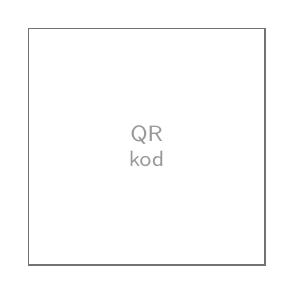
\begin{tikzpicture}
\draw[black!55,line width=0.6pt] (0,0) rectangle (30mm,30mm);
\node[black!40,font=\sffamily\fontsize{8}{9}\selectfont,align=center] at (15mm,15mm) {QR\\kod};
\end{tikzpicture}\\[1.5mm]
{\sffamily\fontsize{9}{11}\selectfont\color{black!70} #1}%
}

% ---- SAT-style multiple-choice question block: #1=number #2=stem #3-6=choices A-D ----
\newcommand{\satq}[6]{%
\noindent\pnum{#1} #2\\[2mm]
\hspace*{7mm}\begin{tabular}{@{}p{32mm}p{32mm}@{}}
(A) #3 & (B) #4 \\[2.5mm]
(C) #5 & (D) #6 \\
\end{tabular}\\[7mm]%
}

\arrayrulecolor{accent}
\setlength{\arrayrulewidth}{0.7pt}
\renewcommand{\arraystretch}{1.35}
\newcommand{\anstitle}[1]{{\sffamily\bfseries\color{accent}\fontsize{11}{13}\selectfont #1}\\[1.3mm]}

\begin{document}

% ================= PAGE 1: Set 1 | Set 2 =================
\topicheader{7}{Daraja va Ildizlar}
\pagefooter{45}
\colrule{32}{238}
\mbox{}%

\begin{textblock*}{\COLW}(\LCOL,32mm)
{\fontsize{12}{15}\selectfont
\setkicker{1-to'plam}{Daraja qoidalari -- nol/manfiy ko'rsatkichsiz sof mashq.}

\noindent\pnum{1} $2^2\times2^3=$\\[22mm]
\noindent\pnum{2} $\dfrac{3^4}{3^2}=$\\[22mm]
\noindent\pnum{3} $(2^2)^3=$\\[22mm]
\noindent\pnum{4} $5^3\times5^2=$\\[22mm]
\noindent\pnum{5} $\dfrac{4^5}{4^3}=$\\[22mm]
\noindent\pnum{6} $(3^2)^2=$\\[22mm]
\noindent\pnum{7} $2^3\times2^3=$\\[22mm]
\noindent\pnum{8} $(2^3)^3=$
}
\end{textblock*}

\begin{textblock*}{\COLW}(\RCOL,32mm)
{\fontsize{12}{15}\selectfont
\setkicker{2-to'plam}{Nol va manfiy ko'rsatkichlar.}

\noindent\pnum{1} $5^0=$\\[22mm]
\noindent\pnum{2} $2^{-3}=$\\[22mm]
\noindent\pnum{3} $4^{-2}=$\\[22mm]
\noindent\pnum{4} $2^0\times2^{-2}=$\\[22mm]
\noindent\pnum{5} $3^{-2}\times3^4=$\\[22mm]
\noindent\pnum{6} $5^2\times5^{-2}=$\\[22mm]
\noindent\pnum{7} $10^{-1}\times100=$\\[22mm]
\noindent\pnum{8} $2^{-1}+2^{-2}=$
}
\end{textblock*}

\clearpage

% ================= PAGE 2: Set 3 | Set 4 =================
\topicheader{7}{Daraja va Ildizlar}
\pagefooter{46}
\colrule{32}{238}
\mbox{}%

\begin{textblock*}{\COLW}(\LCOL,32mm)
{\fontsize{12}{15}\selectfont
\setkicker{3-to'plam}{Aralash -- haqiqiy test zichligi.}

\noindent\pnum{1} $\dfrac{(2^2\times2^3)^2}{2^4}=$\\[22mm]
\noindent\pnum{2} $(3\times3^2)^2=$\\[22mm]
\noindent\pnum{3} $\dfrac{5^3}{5^2\times5^{-1}}=$\\[22mm]
\noindent\pnum{4} $(2^{-1})^{-3}=$\\[22mm]
\noindent\pnum{5} $(4^2)^0=$\\[22mm]
\noindent\pnum{6} $\dfrac{2^5}{2^{-2}}=$\\[22mm]
\noindent\pnum{7} $\dfrac{(3^2)^2}{3^3}=$\\[22mm]
\noindent\pnum{8} $10^3\times10^{-1}\div10=$
}
\end{textblock*}

\begin{textblock*}{\COLW}(\RCOL,32mm)
{\fontsize{12}{15}\selectfont
\setkicker{4-to'plam}{Kvadrat ildizlarni soddalashtirish.}

\noindent\pnum{1} $\sqrt{16}=$\\[22mm]
\noindent\pnum{2} $\sqrt{49}=$\\[22mm]
\noindent\pnum{3} $\sqrt{18}=$\\[22mm]
\noindent\pnum{4} $\sqrt{50}=$\\[22mm]
\noindent\pnum{5} $\sqrt{72}=$\\[22mm]
\noindent\pnum{6} $\sqrt{20}=$\\[22mm]
\noindent\pnum{7} $\sqrt{45}=$\\[22mm]
\noindent\pnum{8} $\sqrt{8}=$
}
\end{textblock*}

\clearpage

% ================= PAGE 3: Set 5 | Set 6 (spot the error) =================
\topicheader{7}{Daraja va Ildizlar}
\pagefooter{47}
\colrule{32}{238}
\mbox{}%

\begin{textblock*}{\COLW}(\LCOL,32mm)
{\fontsize{12}{15}\selectfont
\setkicker{5-to'plam}{Ildizlarni qo'shish va ayirish.}

\noindent\pnum{1} $\sqrt{8}+\sqrt{2}=$\\[22mm]
\noindent\pnum{2} $\sqrt{18}-\sqrt{2}=$\\[22mm]
\noindent\pnum{3} $\sqrt{12}+\sqrt{27}=$\\[22mm]
\noindent\pnum{4} $\sqrt{50}-\sqrt{8}=$\\[22mm]
\noindent\pnum{5} $2\sqrt{3}\times\sqrt{3}=$\\[22mm]
\noindent\pnum{6} $\sqrt{2}\times\sqrt{8}=$\\[22mm]
\noindent\pnum{7} $3\sqrt{5}+2\sqrt{5}=$\\[22mm]
\noindent\pnum{8} $\sqrt{45}-\sqrt{20}=$
}
\end{textblock*}

\begin{textblock*}{\COLW}(\RCOL,32mm)
{\fontsize{11}{14}\selectfont
\setkicker{6-to'plam}{Xatoni toping -- buzilgan qadamni ayting, to'g'ri javobni bering.}

\noindent\pnum{1} $2^3\times2^3$ ifodasida ko'rsatilgan yechimda xato bor:\\[1mm]
\hspace*{7mm}\textit{``$2^3\times2^3=2^9=512$.''}\\[2mm]
\hspace*{7mm}Xato va to'g'ri javob: \makebox[52mm]{\dotfill}\\[10mm]

\noindent\pnum{2} $(2^2)^3$ ifodasida ko'rsatilgan yechimda xato bor:\\[1mm]
\hspace*{7mm}\textit{``$(2^2)^3=2^{2+3}=2^5=32$.''}\\[2mm]
\hspace*{7mm}Xato va to'g'ri javob: \makebox[52mm]{\dotfill}\\[10mm]

\noindent\pnum{3} $2^{-3}$ ifodasida ko'rsatilgan yechimda xato bor:\\[1mm]
\hspace*{7mm}\textit{``$2^{-3}=-8$.''}\\[2mm]
\hspace*{7mm}Xato va to'g'ri javob: \makebox[52mm]{\dotfill}\\[10mm]

\noindent\pnum{4} $\sqrt{16+9}$ ifodasida ko'rsatilgan yechimda xato bor:\\[1mm]
\hspace*{7mm}\textit{``$\sqrt{16}+\sqrt{9}=4+3=7$.''}\\[2mm]
\hspace*{7mm}Xato va to'g'ri javob: \makebox[52mm]{\dotfill}\\[10mm]

\noindent\pnum{5} $\sqrt{32}$ ifodasida ko'rsatilgan yechimda xato bor:\\[1mm]
\hspace*{7mm}\textit{``$32=16\times2$ deb to'g'ri ajratilgan, lekin javobda $16\sqrt2$ deb yozilgan.''}\\[2mm]
\hspace*{7mm}Xato va to'g'ri javob: \makebox[52mm]{\dotfill}
}
\end{textblock*}

\clearpage

% ================= PAGE 4: Set 7 (bonus) =================
\topicheader{7}{Daraja va Ildizlar}
\pagefooter{48}
\colrule{32}{238}
\mbox{}%

\begin{textblock*}{\COLW}(\LCOL,32mm)
{\fontsize{12}{15}\selectfont
\setkicker{7-to'plam}{Bonus / qiyin -- har biriga taxminan 90 soniya.}

\noindent\pnum{1} $\dfrac{(2^3)^2}{2^4}+\sqrt{16}=$\\[26mm]
\noindent\pnum{2} $\sqrt{3^2\times2^2}=$\\[26mm]
\noindent\pnum{3} $2^{-2}\times4^2+\sqrt{9}=$\\[26mm]
\noindent\pnum{4} $(\sqrt{2})^4=$\\[26mm]
\noindent\pnum{5} $1+\sqrt{5^2-3^2}=$
}
\end{textblock*}

\clearpage

% ================= PAGE 5: Set 8 (SAT-style application, MC) -- own page =================
\topicheader{7}{Daraja va Ildizlar}
\pagefooter{49}
\colrule{32}{238}
\mbox{}%

\begin{textblock*}{\COLW}(\LCOL,32mm)
{\fontsize{10.5}{13}\selectfont
\setkicker{8-to'plam}{SAT'da qanday uchraydi -- daraja va ildiz qoidalarini qo'llash.}

\satq{1}{$2^3\times2^4$ ifodaning qiymati nechaga teng?}{128}{64}{16}{81}
\satq{2}{$\dfrac{5^6}{5^2}$ ifodaning qiymati nechaga teng?}{25}{625}{125}{15625}
\satq{3}{$(x^3)^4$ ifodasi barcha $x$ uchun qaysi ifodaga teng?}{$x^7$}{$x^{64}$}{$x^{12}$}{$x^{81}$}
\satq{4}{$7^0+3^2$ ifodaning qiymati nechaga teng?}{9}{16}{19}{10}
\satq{5}{$4^{-2}$ ifodaning qiymati nechaga teng?}{$\dfrac{1}{16}$}{$-8$}{$-16$}{16}
\satq{6}{Agar $a=2^5$ va $b=2^3$ bo'lsa, $\dfrac{a}{b}$ nechaga teng?}{2}{4}{8}{16}
}
\end{textblock*}

\begin{textblock*}{\COLW}(\RCOL,32mm)
{\fontsize{10.5}{13}\selectfont
\vspace{9mm}

\satq{7}{$\sqrt{98}$ ni eng oddiy ildiz ko'rinishida yozing.}{$14\sqrt2$}{$2\sqrt{49}$}{$7\sqrt2$}{$49\sqrt2$}
\satq{8}{Kvadratning yuzi 48 kvadrat birlikka teng. Uning tomoni (eng oddiy ildiz ko'rinishida) nechaga teng?}{$16\sqrt3$}{$6\sqrt2$}{$2\sqrt{12}$}{$4\sqrt3$}
\satq{9}{$3^4\times3^{-2}$ ifodaning qiymati nechaga teng?}{9}{729}{$\dfrac{1}{9}$}{1}
\satq{10}{$2^n=\dfrac{1}{8}$ tenglamasini qanoatlantiruvchi $n$ qanday qiymatga ega?}{3}{$-3$}{$-8$}{8}
\satq{11}{$\sqrt{45}+\sqrt{20}$ ifodaning qiymati nechaga teng?}{$5\sqrt{65}$}{$\sqrt{65}$}{$5\sqrt5$}{$25\sqrt5$}
\satq{12}{Idishdagi bakteriyalar soni har soatda ikki baravar oshadi. Boshlang'ich son $P_0=2^3$. Yana 2 marta ikki baravar oshgandan keyin, soni (daraja ko'rinishida) nechaga teng?}{$2^6$}{$2^1$}{$2^9$}{$2^5$}
}
\end{textblock*}

\clearpage

% ================= PAGE 6: Javoblar =================
\topicheader{7}{Daraja va Ildizlar}
\pagefooter{50}
\mbox{}%

\begin{textblock*}{194mm}(16mm,30mm)
{\bfseries\itshape\color{accent}\fontsize{19}{21}\selectfont\centering Javoblar\par}
\end{textblock*}

\begin{textblock*}{194mm}(16mm,44mm)
{\fontsize{10}{12.5}\selectfont
\centering
\renewcommand{\arraystretch}{1.3}
\begin{tabular}{|>{\centering\arraybackslash}p{26mm}|>{\centering\arraybackslash}p{10mm}|>{\centering\arraybackslash}p{28mm}|>{\centering\arraybackslash}p{10mm}|>{\centering\arraybackslash}p{28mm}|}
\hline
\rowcolor{badge!55}\textbf{To'plam} & \textbf{\#} & \textbf{Javob} & \textbf{\#} & \textbf{Javob}\\
\hline
\multirow{4}{26mm}{\centering 1-to'plam} & 1 & 32 & 2 & 9\\\cline{2-5}
 & 3 & 64 & 4 & 3125\\\cline{2-5}
 & 5 & 16 & 6 & 81\\\cline{2-5}
 & 7 & 64 & 8 & 512\\\hline
\multirow{4}{26mm}{\centering 2-to'plam} & 1 & 1 & 2 & $\frac{1}{8}$\\\cline{2-5}
 & 3 & $\frac{1}{16}$ & 4 & $\frac{1}{4}$\\\cline{2-5}
 & 5 & 9 & 6 & 1\\\cline{2-5}
 & 7 & 10 & 8 & $\frac{3}{4}$\\\hline
\multirow{4}{26mm}{\centering 3-to'plam} & 1 & 64 & 2 & 729\\\cline{2-5}
 & 3 & 25 & 4 & 8\\\cline{2-5}
 & 5 & 1 & 6 & 128\\\cline{2-5}
 & 7 & 3 & 8 & 10\\\hline
\multirow{4}{26mm}{\centering 4-to'plam} & 1 & 4 & 2 & 7\\\cline{2-5}
 & 3 & $3\sqrt2$ & 4 & $5\sqrt2$\\\cline{2-5}
 & 5 & $6\sqrt2$ & 6 & $2\sqrt5$\\\cline{2-5}
 & 7 & $3\sqrt5$ & 8 & $2\sqrt2$\\\hline
\multirow{4}{26mm}{\centering 5-to'plam} & 1 & $3\sqrt2$ & 2 & $2\sqrt2$\\\cline{2-5}
 & 3 & $5\sqrt3$ & 4 & $3\sqrt2$\\\cline{2-5}
 & 5 & 6 & 6 & 4\\\cline{2-5}
 & 7 & $5\sqrt5$ & 8 & $\sqrt5$\\\hline
\multirow{3}{26mm}{\centering 7-to'plam} & 1 & 8 & 2 & 6\\\cline{2-5}
 & 3 & 7 & 4 & 4\\\cline{2-5}
 & 5 & 5 & -- & --\\\hline
\multirow{6}{26mm}{\centering 8-to'plam} & 1 & A & 2 & B\\\cline{2-5}
 & 3 & C & 4 & D\\\cline{2-5}
 & 5 & A & 6 & B\\\cline{2-5}
 & 7 & C & 8 & D\\\cline{2-5}
 & 9 & A & 10 & B\\\cline{2-5}
 & 11 & C & 12 & D\\\hline
\multirow{5}{26mm}{\centering 6-to'plam} & \multicolumn{4}{p{76mm}|}{1.\ Ko'rsatkichlarni ko'paytirgan, qo'shish kerak edi (ko'paytma qoidasi). To'g'ri: $2^{3+3}=2^6=64$.}\\\cline{2-5}
 & \multicolumn{4}{p{76mm}|}{2.\ Ko'rsatkichlarni qo'shgan, ko'paytirish kerak edi (daraja darajasi). To'g'ri: $2^{2\times3}=2^6=64$.}\\\cline{2-5}
 & \multicolumn{4}{p{76mm}|}{3.\ Manfiy ko'rsatkichni asosni manfiy qiladi deb tushungan. To'g'ri: $2^{-3}=\frac{1}{8}$.}\\\cline{2-5}
 & \multicolumn{4}{p{76mm}|}{4.\ Yig'indining ildizini ildizlar yig'indisiga bo'lgan -- bu hech qachon to'g'ri emas. To'g'ri: $\sqrt{25}=5$.}\\\cline{2-5}
 & \multicolumn{4}{p{76mm}|}{5.\ $16$ ni to'g'ri ajratgan, lekin uning ildizini olmagan. To'g'ri: $\sqrt{16\times2}=4\sqrt2$.}\\\hline
\end{tabular}
}
\end{textblock*}

\begin{textblock*}{194mm}(16mm,240mm)
\centering
{\sffamily\fontsize{9.5}{11.5}\selectfont\color{black!70} Video yechimlar va qo'shimcha testlar uchun quyidagi QR kodlarni skanerlang:}\\[4mm]
\begin{minipage}[t]{32mm}\centering\qrbox{YouTube}\end{minipage}%
\hspace{16mm}%
\begin{minipage}[t]{32mm}\centering\qrbox{Telegram}\end{minipage}
\end{textblock*}

\end{document}
